\documentclass[]{ctexart}
\usepackage[]{graphicx}
\graphicspath{{pictures}}
\title{反馈 Feedback}
\begin{document}

\section{反馈的定义}
\subsection{反馈系统}
    \begin{figure}[ht]
        \centering
        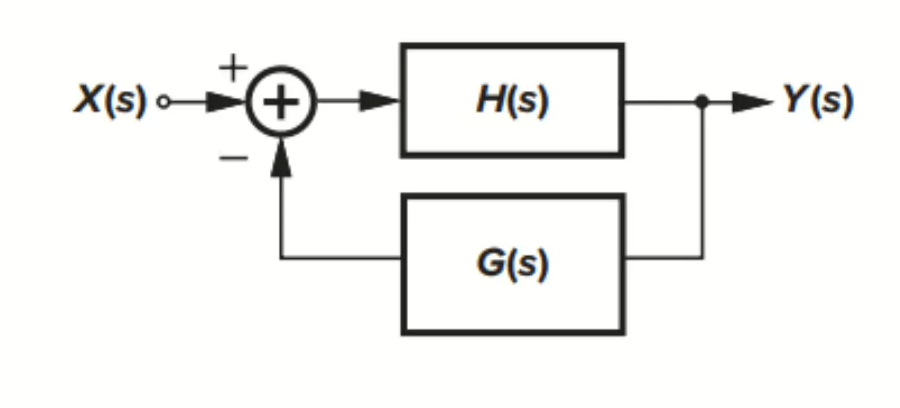
\includegraphics[width=0.75\columnwidth]{Feedback_System}
        \label{图1}
        \caption{反馈系统}
    \end{figure}

    输出信号Y(s)的一部分被G(s)检测,并与输入信号X(s)相比较,产生一个误差项X(s)-G(s)Y(s),即:
    \begin{equation}
        Y(s)=H(s)[X(s)-G(s)Y(s)]
    \end{equation}
    \begin{equation}
        {Y(s) \over X(s)}={H(s) \over 1+G(s)H(s)}
    \end{equation}

    \underline{H(s):开环传输函数 Open-loop Transfer Tunction}

    \underline{Y(s)/X(s):闭环传输函数 Closed-loop Transfer Function}

    \underline{G(s):反馈系数 Feedback Factor}

    \underline{X(s) - G(s)Y(s):反馈误差 Feedback Error}

\subsection{放大电路中的反馈}
    在放大电路中图1可以画成以下这样:

    \begin{figure}[ht]
        \centering
        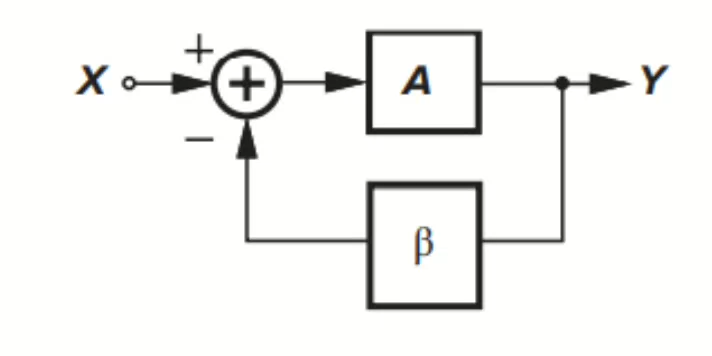
\includegraphics[scale=0.19]{Simple_Feedback_System}
        \label{图2}
        \caption{简单反馈系统}
    \end{figure}

    由图可得:
    \begin{equation}
        Y=A[X-{\beta}Y]
    \end{equation}
    \begin{equation}
        {Y \over X}={A \over 1+{\beta}A}
    \end{equation}

    \underline{A:开环增益 Open-loop Gain}

    \underline{Y/X:闭环增益 Closed-loop Gain}

    \underline{$\beta$:反馈系数 Feedback Factor}

    \underline{$\beta$A:环路增益 Loop Gain (LG)}

\subsection{增益修正}
    通过等式4很显然$\beta$A的值很关键。
\end{document}